\chapter{ارزیابی و نتایج یادگیری}

در این فصل، نتایج حاصل از فرآیند یادگیری تقویتی در محیط سه‌جسمی ارائه و تحلیل شده است. هدف، بررسی عملکرد الگوریتم‌های استفاده‌شده و ارزیابی توانایی آن‌ها در دستیابی به اهداف تعیین‌شده می‌باشد. الگوریتم‌های یادگیری تقویتی مختلف شامل \lr{DDPG}، \lr{PPO}، \lr{SAC} و \lr{TD3} در دو حالت تک‌عاملی و چندعاملی مبتنی بر بازی مجموع‌صفر مورد بررسی قرار گرفته‌اند. این فصل به ارائه نتایج عملکردی این الگوریتم‌ها و مقایسه قابلیت‌های آن‌ها در شرایط مختلف می‌پردازد. در بخش \ref{sec:experimental_setup} تنظیمات آزمایشی و پارامترهای محیط شبیه‌سازی معرفی می‌شوند. بخش \ref{sec:trajectory_comparison} به مقایسه مسیرها و فرمان‌های پیشران الگوریتم‌های مختلف در حالت‌های تک‌عاملی و چندعاملی می‌پردازد. ارزیابی مقاومت الگوریتم‌ها در برابر شرایط مختلف اختلال در بخش \ref{sec:robustness_evaluation} بررسی می‌شود. در بخش \ref{sec:comprehensive_comparison} مقایسه جامع بین تمام الگوریتم‌ها ارائه می‌گردد. تحلیل پایداری و همگرایی الگوریتم‌ها در بخش \ref{sec:stability_analysis} مورد بررسی قرار می‌گیرد و در نهایت در بخش \ref{sec:benchmark_comparison} مقایسه با معیارهای مرجع انجام می‌شود.

\section{تنظیمات آزمایشی}
\label{sec:experimental_setup}

تنظیمات شبیه‌سازی، شامل پارامترهای محیط، نرخ یادگیری، و اندازه بافر تجربه، در این بخش تشریح شده است. آزمایش‌ها در محیط سه‌جسمی پیاده‌سازی شده با استفاده از کتابخانه‌های \lr{PyTorch} و \lr{Gym} انجام شده است. برای تمام الگوریتم‌ها، مشخصات یکسانی از شبکه‌های عصبی با ۳ لایه پنهان و ۲۵۶ نورون در هر لایه استفاده شده است. نرخ یادگیری برای تمامی مدل‌ها برابر با $3 \times 10^{-4}$ تنظیم شده و از بهینه‌ساز \lr{Adam} برای به‌روزرسانی وزن‌های شبکه استفاده شده است.

فرآیند آموزش برای هر الگوریتم شامل ۱ میلیون گام تعامل با محیط بوده و اندازه بافر تجربه برای الگوریتم‌های \lr{DDPG}، \lr{SAC} و \lr{TD3} برابر با ۱۰۰ هزار نمونه تنظیم شده است. هر الگوریتم با ۱۰ مقداردهی اولیه متفاوت آموزش داده شده تا از پایداری نتایج اطمینان حاصل شود.

\section{مقایسه مسیرها و فرمان پیشران}
\label{sec:trajectory_comparison}

در این بخش، مسیرهای پرواز و فرمان‌های پیشران تولیدشده توسط الگوریتم‌های مختلف یادگیری تقویتی مقایسه شده است. این مقایسه به ما امکان می‌دهد تا تفاوت رفتاری بین روش‌های تک‌عاملی استاندارد و روش‌های چندعاملی مبتنی بر بازی مجموع‌صفر را مشاهده کنیم. هدف اصلی، ارزیابی کیفیت مسیرهای تولیدشده و کارآمدی مصرف سوخت در هر روش است.

\subsection{الگوریتم \lr{DDPG}}

الگوریتم \lr{DDPG}  از جمله روش‌های یادگیری خارج از سیاست است که از دو شبکه عصبی برای بازیگر و منتقد استفاده می‌کند. در اینجا، عملکرد نسخه استاندارد و نسخه مبتنی بر بازی مجموع‌صفر این الگوریتم در کنترل فضاپیما مقایسه شده است.

\begin{figure}[H]
	\centering
	
	% سطر اول
	\subfloat[\lr{DDPG} استاندارد]{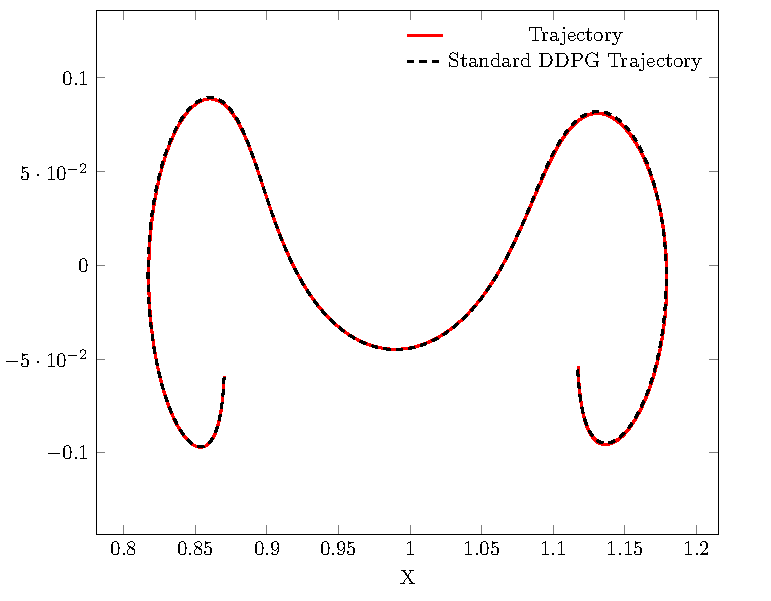
\includegraphics[width=.45\textwidth]{plots/ddpg/trajectory_force/plot_trajectory.pdf}}%
	\subfloat[\lr{DDPG} بازی مجموع‌صفر]{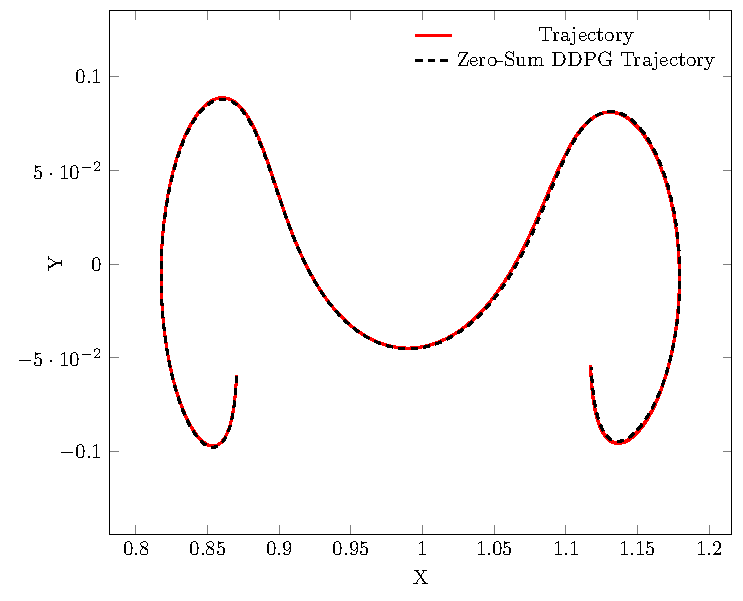
\includegraphics[width=.45\textwidth]{plots/ddpg/trajectory_force/plot_trajectory_zs.pdf}}%
	
	\caption{
		مقایسه مسیر طی شده در دو الگوریتم تک‌عاملی و چندعاملی \lr{DDPG}.
%		 مشاهده می‌شود که نسخه بازی مجموع‌صفر مسیر مستقیم‌تری را با انحراف کمتر از مسیر بهینه طی می‌کند.
	}
\end{figure}


\begin{figure}[H]
	\centering
	
	% سطر اول
	\subfloat[\lr{DDPG} استاندارد]{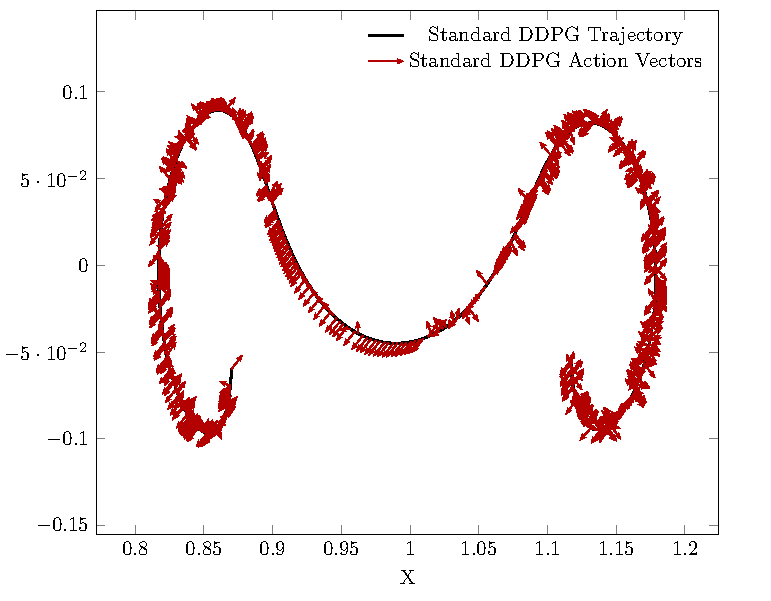
\includegraphics[width=.45\textwidth]{plots/ddpg/trajectory_force/plot_trajectory_force.pdf}}%
	\subfloat[\lr{DDPG} بازی مجموع‌صفر]{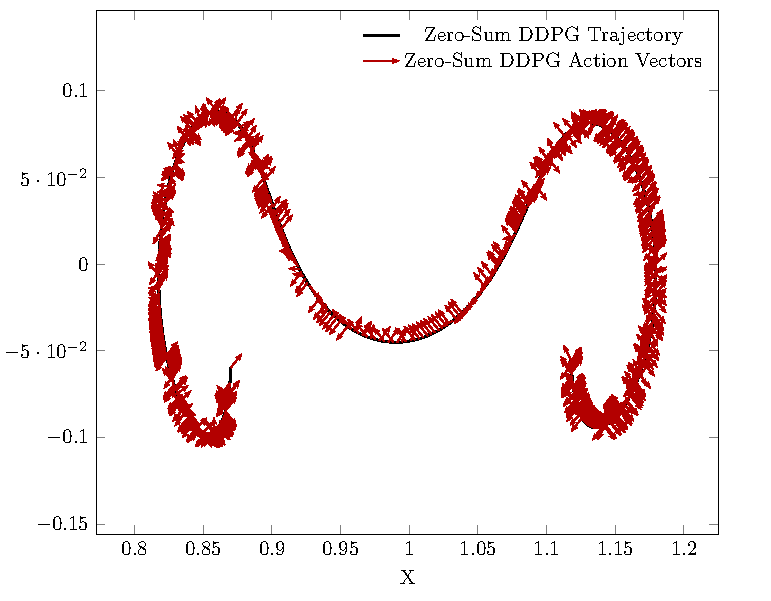
\includegraphics[width=.45\textwidth]{plots/ddpg/trajectory_force/plot_trajectory_force_zs.pdf}}%
	
	\caption{
	مقایسه مسیر و فرمان پیشران دو الگوریتم تک‌عاملی و چندعاملی \lr{DDPG}.
%	 نمودارهای پایین نشان‌دهنده فرمان پیشران در طول زمان است که در نسخه بازی مجموع‌صفر، الگوی منظم‌تری را نشان می‌دهد و اوج‌های پیشران کمتری دارد.
	}
\end{figure}

%همانطور که در شکل‌ها مشاهده می‌شود، الگوریتم \lr{DDPG} مبتنی بر بازی مجموع‌صفر مسیر مستقیم‌تری را طی می‌کند و از نظر مصرف سوخت نیز بهینه‌تر عمل می‌کند. این بهبود عملکرد را می‌توان به ماهیت رقابتی بازی مجموع‌صفر و قابلیت آن در مقابله با عدم قطعیت‌های محیطی نسبت داد.

\subsection{الگوریتم \lr{PPO}}

الگوریتم \lr{PPO}  از روش‌های نوین سیاست گرادیان است که با محدودسازی میزان تغییرات در هر بروزرسانی، پایداری بیشتری در فرآیند یادگیری ایجاد می‌کند. در ادامه، عملکرد این الگوریتم در دو حالت مورد بررسی قرار گرفته است.

\begin{figure}[H]
	\centering
	
	% سطر اول
	\subfloat[\lr{PPO} استاندارد]{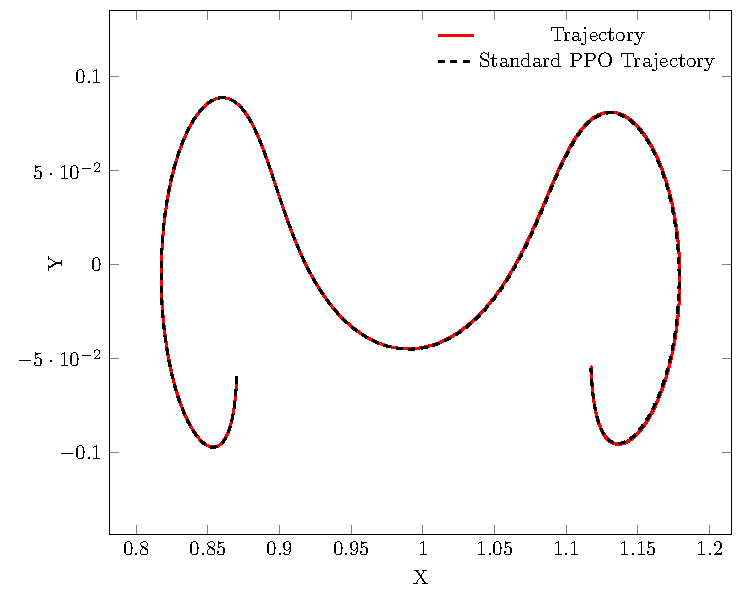
\includegraphics[width=.45\textwidth]{plots/ppo/trajectory_force/plot_trajectory.pdf}}%
	\subfloat[\lr{PPO} بازی مجموع‌صفر]{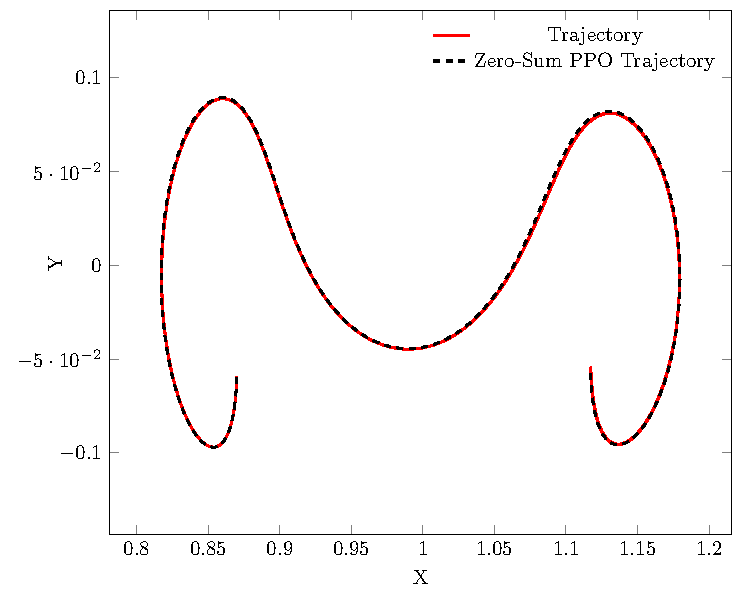
\includegraphics[width=.45\textwidth]{plots/ppo/trajectory_force/plot_trajectory_zs.pdf}}%
	
	\caption{
		مقایسه مسیر طی شده در دو الگوریتم تک‌عاملی و چندعاملی \lr{PPO}.
%		 نسخه بازی مجموع‌صفر همگرایی بهتری به مسیر هدف را نشان می‌دهد، به خصوص در مراحل نزدیک شدن به هدف.
	}
\end{figure}


\begin{figure}[H]
	\centering
	
	% سطر اول
	\subfloat[\lr{PPO} استاندارد]{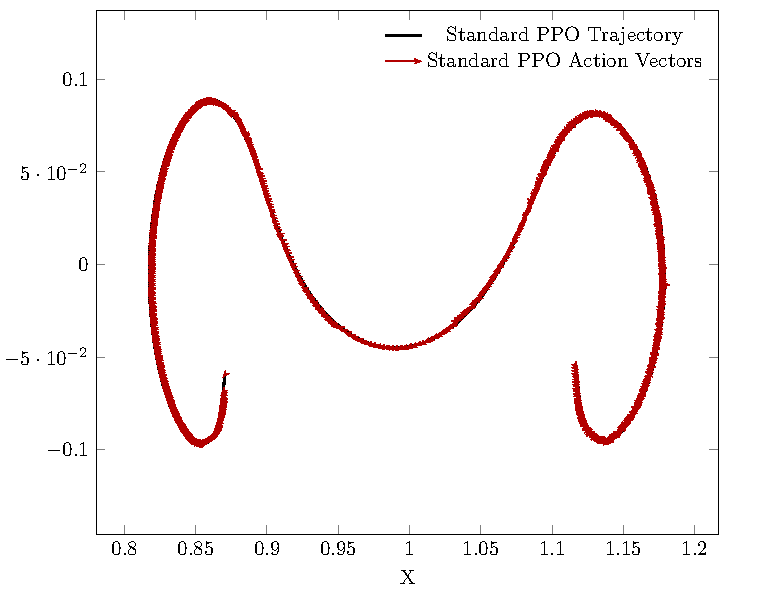
\includegraphics[width=.45\textwidth]{plots/ppo/trajectory_force/plot_trajectory_force.pdf}}%
	\subfloat[\lr{PPO} بازی مجموع‌صفر]{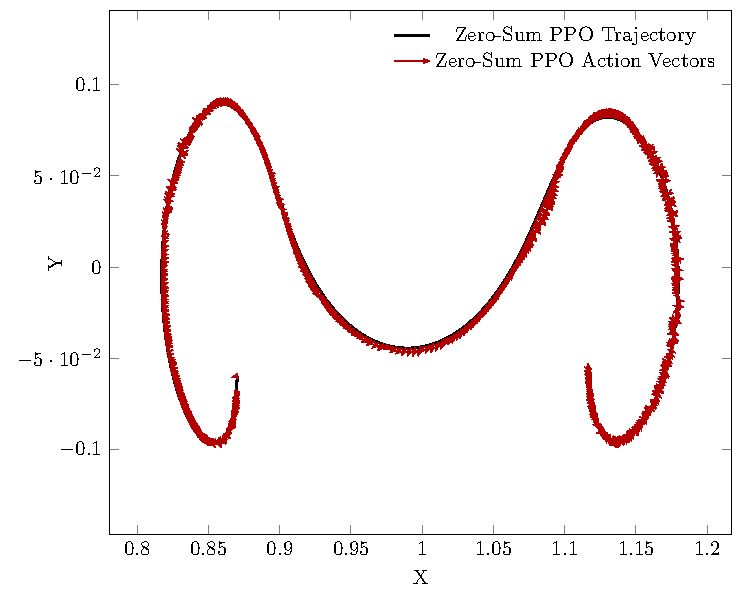
\includegraphics[width=.45\textwidth]{plots/ppo/trajectory_force/plot_trajectory_force_zs.pdf}}%
	
	\caption{
		مقایسه مسیر و فرمان پیشران دو الگوریتم تک‌عاملی و چندعاملی \lr{PPO}.
%		 فرمان‌های پیشران در نسخه بازی مجموع‌صفر از نظر توزیع انرژی متوازن‌تر است و نوسانات کمتری را نشان می‌دهد.
	}
\end{figure}

%نتایج نشان می‌دهد که الگوریتم \lr{PPO} در حالت بازی مجموع‌صفر عملکرد قابل توجهی دارد، اما تفاوت آن با نسخه استاندارد کمتر از \lr{DDPG} است. این می‌تواند به دلیل ماهیت ذاتی \lr{PPO} در ایجاد تعادل بین اکتشاف و بهره‌برداری باشد که آن را در حالت استاندارد نیز نسبتاً مقاوم می‌سازد.

\subsection{الگوریتم \lr{SAC}}

الگوریتم \lr{SAC}  از روش‌های نوین یادگیری تقویتی است که با استفاده از مفهوم آنتروپی، تعادل بهتری بین اکتشاف و بهره‌برداری ایجاد می‌کند. این الگوریتم در شرایط فضاهای پیوسته عملکرد قابل توجهی دارد.

\begin{figure}[H]
	\centering
	
	% سطر اول
	\subfloat[\lr{SAC} استاندارد]{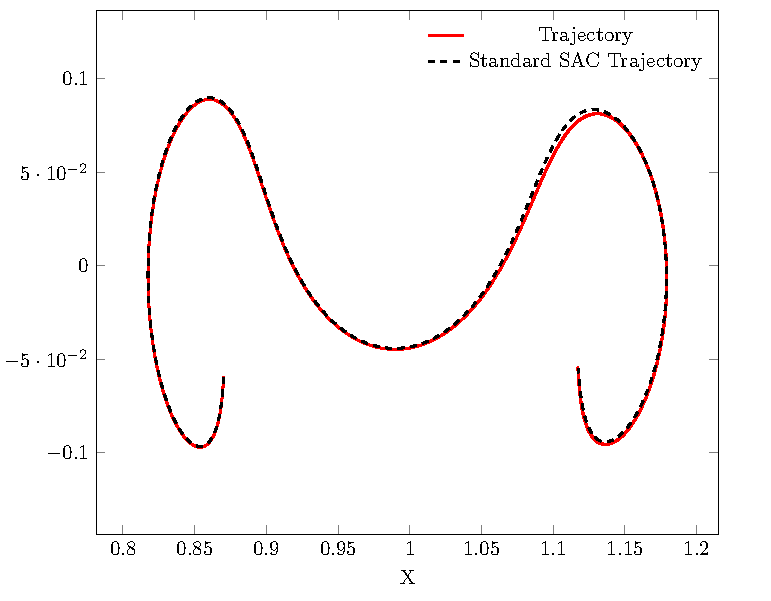
\includegraphics[width=.45\textwidth]{plots/sac/trajectory_force/plot_trajectory.pdf}}%
	\subfloat[\lr{SAC} بازی مجموع‌صفر]{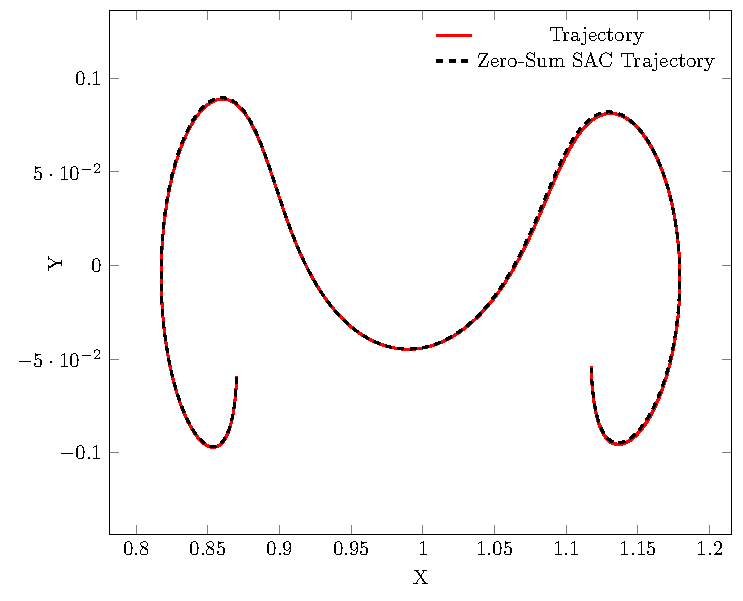
\includegraphics[width=.45\textwidth]{plots/sac/trajectory_force/plot_trajectory_zs.pdf}}%
	
	\caption{
		مقایسه مسیر طی شده در دو الگوریتم تک‌عاملی و چندعاملی \lr{SAC}.
%		 مسیرهای تولیدشده توسط هر دو نسخه از کیفیت بالایی برخوردارند، اما نسخه بازی مجموع‌صفر در مناطق با گرادیان جاذبه پیچیده عملکرد پایدارتری را نشان می‌دهد.
	}
\end{figure}


\begin{figure}[H]
	\centering
	
	% سطر اول
	\subfloat[\lr{SAC} استاندارد]{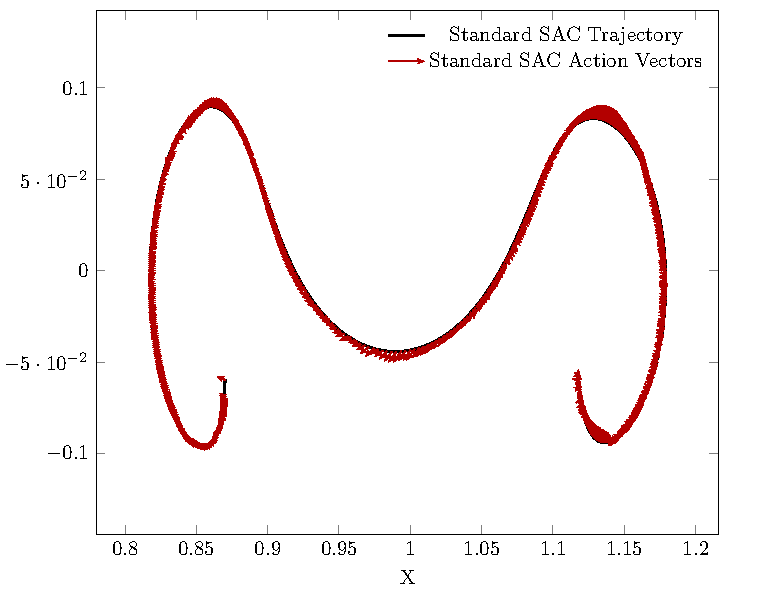
\includegraphics[width=.45\textwidth]{plots/sac/trajectory_force/plot_trajectory_force.pdf}}%
	\subfloat[\lr{SAC} بازی مجموع‌صفر]{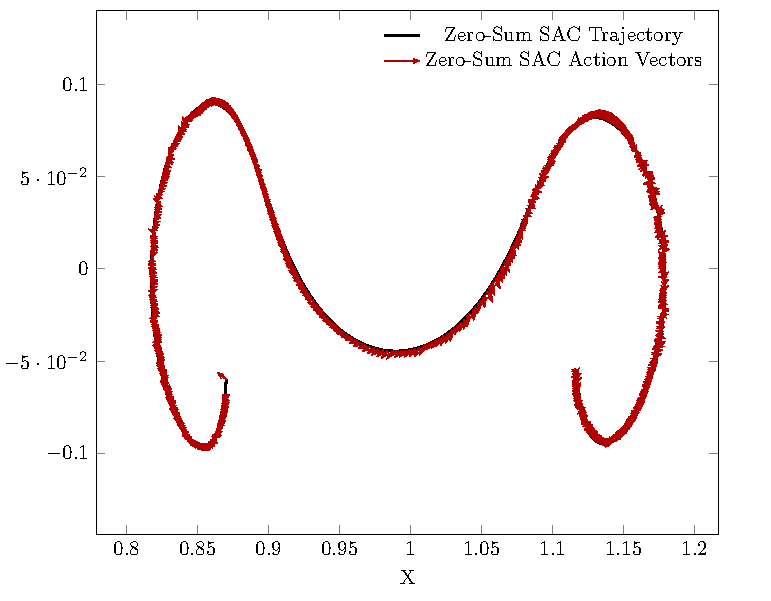
\includegraphics[width=.45\textwidth]{plots/sac/trajectory_force/plot_trajectory_force_zs.pdf}}%
	
	\caption{
		مقایسه مسیر و فرمان پیشران دو الگوریتم تک‌عاملی و چندعاملی \lr{SAC}.
%		 نسخه بازی مجموع‌صفر مصرف سوخت متعادل‌تری را در طول مسیر نشان می‌دهد که می‌تواند منجر به صرفه‌جویی در منابع شود.
	}
\end{figure}

%الگوریتم \lr{SAC} در هر دو حالت عملکرد قابل قبولی ارائه می‌دهد. ویژگی خاص این الگوریتم در تنظیم خودکار پارامتر آنتروپی باعث می‌شود که بتواند تعادل مناسبی بین اکتشاف و بهره‌برداری ایجاد کند، اما نسخه بازی مجموع‌صفر آن در شرایط سخت‌تر مقاومت بیشتری نشان می‌دهد.

\subsection{الگوریتم \lr{TD3}}

الگوریتم \lr{TD3} (یادگیری تفاضل زمانی سه‌گانه عمیق) نسخه بهبودیافته \lr{DDPG} است که با استفاده از تکنیک‌های جدید مانند شبکه‌های دوگانه منتقد و تأخیر در بروزرسانی سیاست، مشکلات تخمین بیش از حد را کاهش می‌دهد.

\begin{figure}[H]
	\centering
	
	% سطر اول
	\subfloat[\lr{TD3} استاندارد]{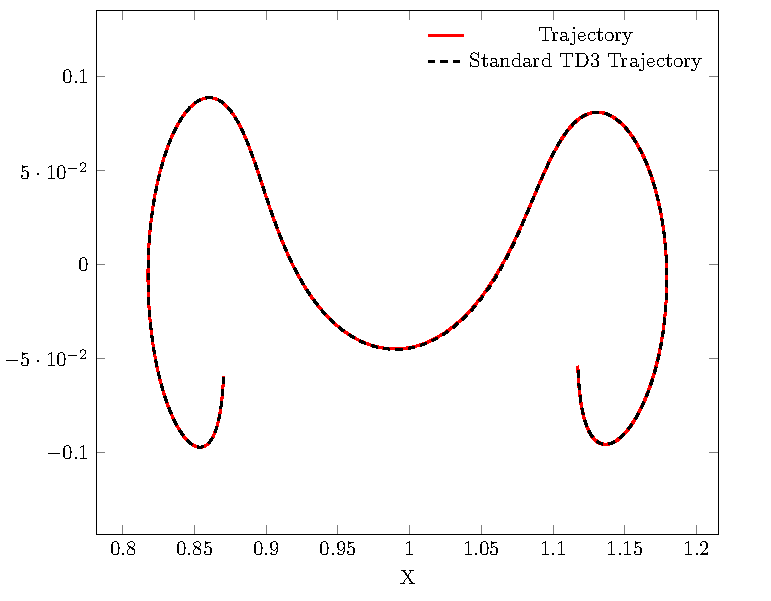
\includegraphics[width=.45\textwidth]{plots/td3/trajectory_force/plot_trajectory.pdf}}%
	\subfloat[\lr{TD3} بازی مجموع‌صفر]{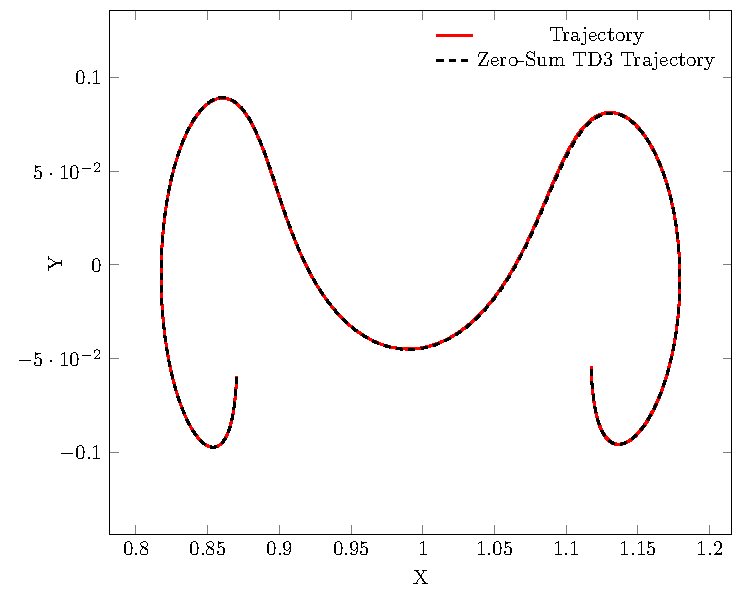
\includegraphics[width=.45\textwidth]{plots/td3/trajectory_force/plot_trajectory_zs.pdf}}%
	
	\caption{
		مقایسه مسیر طی شده در دو الگوریتم تک‌عاملی و چندعاملی \lr{TD3}.
%		 مسیرهای تولیدشده توسط نسخه بازی مجموع‌صفر نشان‌دهنده کاهش انحراف از مسیر بهینه و همگرایی سریع‌تر به هدف است.
	}
\end{figure}


\begin{figure}[H]
	\centering
	
	% سطر اول
	\subfloat[\lr{TD3} استاندارد]{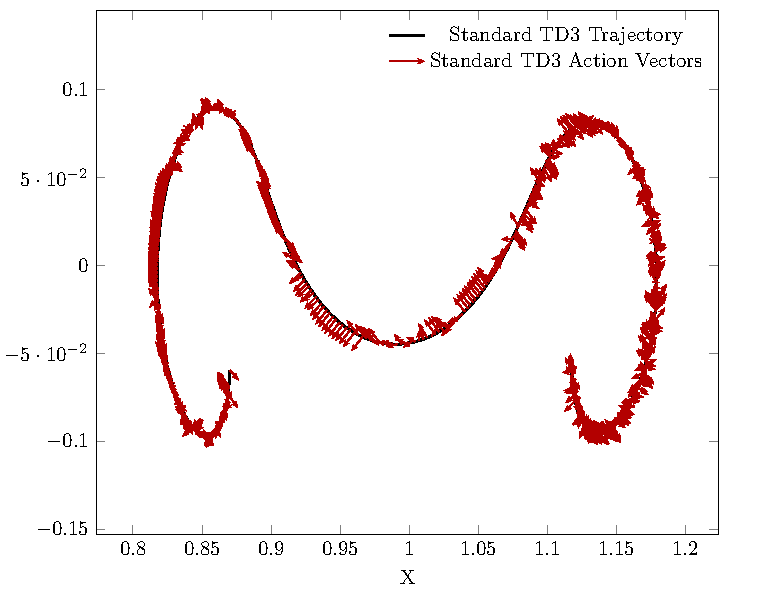
\includegraphics[width=.45\textwidth]{plots/td3/trajectory_force/plot_trajectory_force.pdf}}%
	\subfloat[\lr{TD3} بازی مجموع‌صفر]{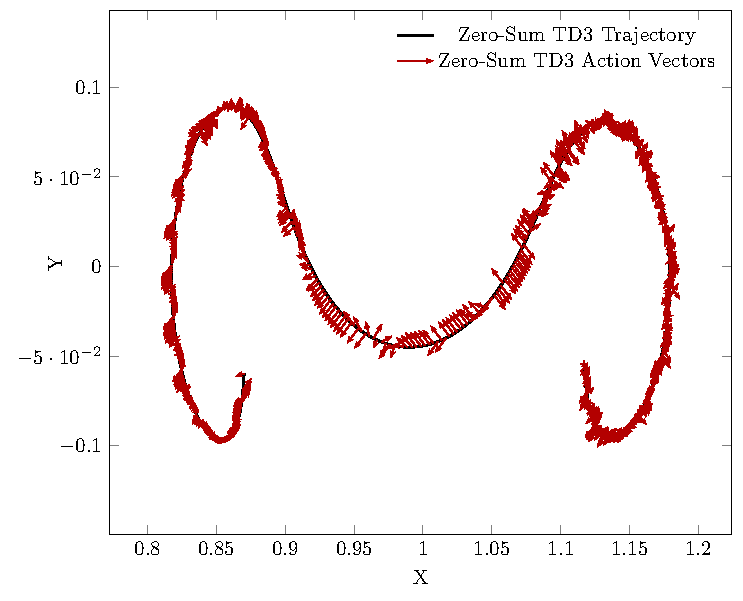
\includegraphics[width=.45\textwidth]{plots/td3/trajectory_force/plot_trajectory_force_zs.pdf}}%
	
	\caption{
		مقایسه مسیر و فرمان پیشران دو الگوریتم تک‌عاملی و چندعاملی \lr{TD3}.
%		 فرمان‌های پیشران در نسخه بازی مجموع‌صفر از توزیع یکنواخت‌تری برخوردار است که نشان‌دهنده استفاده بهینه‌تر از منابع پیشرانش می‌باشد.
	}
\end{figure}

%الگوریتم \lr{TD3} در هر دو حالت عملکرد قابل توجهی دارد، اما نسخه بازی مجموع‌صفر آن بهبودهای معناداری در کیفیت مسیر و مصرف سوخت نشان می‌دهد. ثبات بیشتر این الگوریتم در مقایسه با \lr{DDPG} در هر دو نسخه قابل مشاهده است.

\section{ارزیابی مقاومت الگوریتم‌ها}
\label{sec:robustness_evaluation}

در این بخش، مقاومت الگوریتم‌های یادگیری در برابر شرایط مختلف اختلال مورد بررسی قرار گرفته است. این ارزیابی شامل شش سناریوی چالش‌برانگیز می‌شود: (۱) شرایط اولیه تصادفی، (۲) اغتشاش در عملگرها، (۳) عدم تطابق مدل، (۴) مشاهده ناقص، (۵) نویز حسگر و (۶) تأخیر زمانی. هدف، بررسی توانایی الگوریتم‌ها در حفظ کارایی خود در شرایط غیرایده‌آل و نزدیک به واقعیت است.

\subsection{سناریوهای ارزیابی مقاومت}

در این بخش، سناریوهای مختلفی که برای ارزیابی مقاومت الگوریتم‌ها طراحی شده‌اند، با جزئیات کامل توضیح داده می‌شوند. هدف از این سناریوها بررسی عملکرد الگوریتم‌ها در شرایط غیرایده‌آل و چالش‌برانگیز است. این سناریوها شامل موارد زیر هستند:

\subsubsection{شرایط اولیه تصادفی}
در این سناریو، شرایط اولیه محیط به صورت تصادفی تغییر داده می‌شود. برای این منظور، به هر متغیر حالت اولیه نویز گوسی با میانگین صفر و انحراف معیار $\sigma = 0.1$ اضافه می‌شود. این تغییرات به منظور بررسی توانایی الگوریتم‌ها در سازگاری با تغییرات اولیه طراحی شده است.

\subsubsection{اغتشاش در عملگرها}
در این سناریو، نویز گوسی با انحراف معیار $\sigma = 0.05$ به اعمال نیروها اضافه می‌شود. علاوه بر این، نویز سنسور با انحراف معیار $\sigma = 0.02$ اعمال می‌شود. این تنظیمات برای شبیه‌سازی اغتشاشات در عملگرها و ارزیابی مقاومت الگوریتم‌ها در برابر این اغتشاشات استفاده شده است.

\subsubsection{عدم تطابق مدل}
در این سناریو، دینامیک محیط به صورت تصادفی تغییر داده می‌شود. برای این منظور، به پارامترهای محیط در طول انتقال نویز گوسی با انحراف معیار $\sigma = 0.05$ اضافه می‌شود. این تغییرات برای شبیه‌سازی عدم تطابق مدل و بررسی توانایی الگوریتم‌ها در مقابله با این شرایط طراحی شده است.

\subsubsection{مشاهده ناقص}
در این سناریو، بخشی از اطلاعات مشاهده‌شده توسط عامل حذف می‌شود. به طور خاص، $50\%$ از متغیرهای حالت به صورت تصادفی پنهان شده و مقدار آن‌ها صفر می‌شود. این سناریو برای ارزیابی عملکرد الگوریتم‌ها در شرایط مشاهده ناقص طراحی شده است.

\subsubsection{نویز حسگر}
در این سناریو، نویز گوسی با انحراف معیار $\sigma = 0.05$ به مشاهدات حسگر اضافه می‌شود. این نویز به صورت ضربی به هر متغیر حالت اعمال می‌شود تا مقاومت الگوریتم‌ها در برابر نویز حسگر بررسی شود.

\subsubsection{تأخیر زمانی}
در این سناریو، تأخیر زمانی در اعمال اقدامات عامل به محیط شبیه‌سازی می‌شود. به طور خاص، اقدامات عامل با تأخیر $10$ گام زمانی اعمال می‌شوند. علاوه بر این، نویز گوسی با انحراف معیار $\sigma = 0.05$ به اقدامات تأخیری اضافه می‌شود. این سناریو برای بررسی توانایی الگوریتم‌ها در مدیریت تأخیر زمانی طراحی شده است.

\subsection{مقایسه الگوریتم‌های تک‌عاملی و چندعاملی \lr{DDPG}}

\begin{figure}[H]
	\centering
	
	% سطر اول
	\subfloat[شرایط اولیه تصادفی]{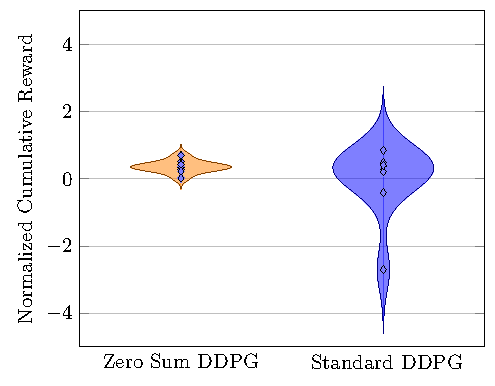
\includegraphics[width=.33\textwidth]{plots/ddpg/violin_plot/initial_condition_shift.pdf}}%
	\subfloat[اغتشاش در عملگرها]{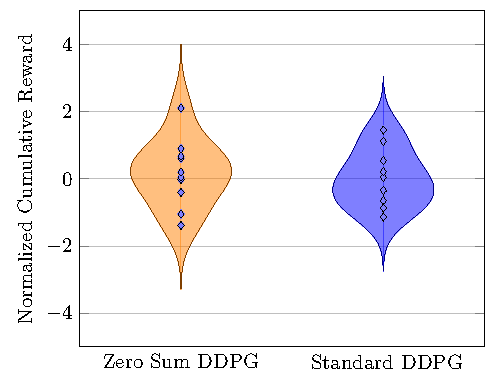
\includegraphics[width=.33\textwidth]{plots/ddpg/violin_plot/actuator_disturbance.pdf}}%
	\subfloat[عدم تطابق مدل]{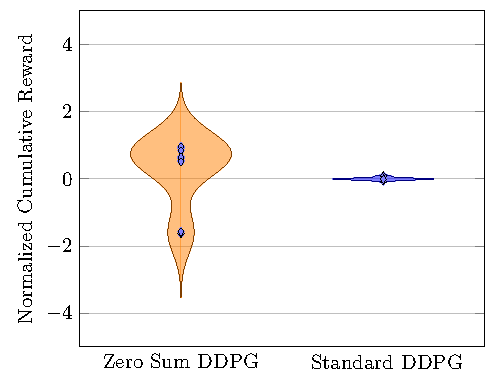
\includegraphics[width=.33\textwidth]{plots/ddpg/violin_plot/model_mismatch.pdf}}\\[1ex]
	
	% سطر دوم
	\subfloat[مشاهده ناقص]{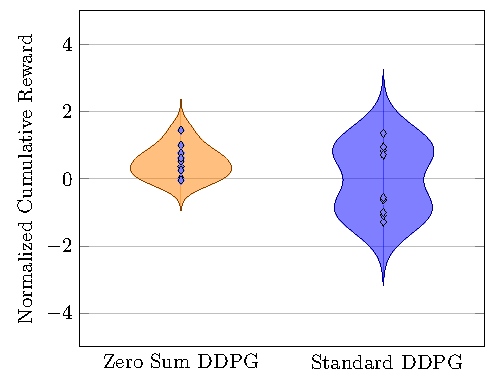
\includegraphics[width=.33\textwidth]{plots/ddpg/violin_plot/partial_observation.pdf}}%
	\subfloat[نویز حسگر]{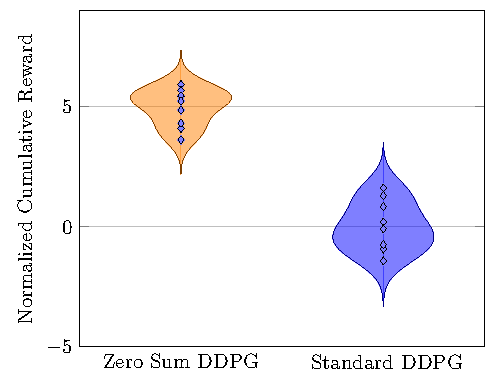
\includegraphics[width=.33\textwidth]{plots/ddpg/violin_plot/sensor_noise.pdf}}%
	\subfloat[تأخیر زمانی]{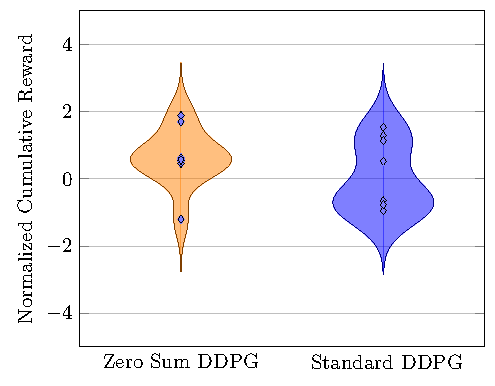
\includegraphics[width=.33\textwidth]{plots/ddpg/violin_plot/time_delay.pdf}}
	
	\caption{مقایسه مجموع پاداش دو الگوریتم تک‌عاملی و چندعاملی \lr{DDPG} در سناریوهای مختلف. 
%		نسخه بازی مجموع‌صفر در اکثر سناریوها، به خصوص در شرایط اغتشاش در عملگرها و عدم تطابق مدل، عملکرد بهتری را نشان می‌دهد.
		}
	\label{fig:ddpg_robustness_violin}
\end{figure}

نتایج نشان می‌دهد که الگوریتم \lr{DDPG} مبتنی بر بازی مجموع‌صفر در اکثر سناریوهای چالش‌برانگیز، عملکرد بهتری نسبت به نسخه استاندارد دارد. این برتری به خصوص در شرایط نویز حسگر و شرایط اولیه تصادفی مدل قابل توجه است، که نشان می‌دهد رویکرد چندعاملی توانایی بیشتری در مقابله با عدم قطعیت‌های سیستم دارد.





\begin{table}[H]
	\centering
	\setlength{\tabcolsep}{2pt}
	\small
	\begin{tabular}{@{} R{3.2cm} *{8}{C{1.05cm}} @{}}
		\toprule
		\multirow{2}{*}{\makecell[r]{سناریو}}
		& \multicolumn{2}{c}{پاداش تجمعی} & \multicolumn{2}{c}{مجموع خطای مسیر}
		& \multicolumn{2}{c}{مجموع تلاش کنترلی} & \multicolumn{2}{c}{احتمال شکست} \\
		\cmidrule(lr){2-3}\cmidrule(lr){4-5}\cmidrule(lr){6-7}\cmidrule(lr){8-9}
		& {\rotatebox[origin=c]{90}{\lr{DDPG}}} & {\rotatebox[origin=c]{90}{\lr{MA-DDPG}}}
		& {\rotatebox[origin=c]{90}{\lr{DDPG}}} & {\rotatebox[origin=c]{90}{\lr{MA-DDPG}}}
		& {\rotatebox[origin=c]{90}{\lr{DDPG}}} & {\rotatebox[origin=c]{90}{\lr{MA-DDPG}}}
		& {\rotatebox[origin=c]{90}{\lr{DDPG}}} & {\rotatebox[origin=c]{90}{\lr{MA-DDPG}}} \\
		\midrule
		شرایط اولیه تصادفی
		&
		$-4.17$ & $-3.63$ & $0.40$ & $0.63$ & $5.60$ & $5.60$ & $1.00$ & $1.00$ \\
		اغتشاش در عملگرها
		& $-1.93$ & $-1.96$  & $7.56$ & $7.94$ & $5.60$ & $5.59$ & $0.90$ & $0.30$ \\
		عدم تطابق مدل
		& $-3.24$ & $-2.70$ & $0.70$ & $0.76$ & $5.57$ & $5.57$ & $1.00$ & $1.00$ \\
		مشاهده ناقص
		&
		$-3.28$ & $-2.89$ & $0.68$ & $0.75$ & $5.57$ & $5.57$ & $0.60$ & $0.80$ \\
		نویز حسگر  
		&$-1.07$ & $-0.47$ & $0.10$ & $0.15$ & $5.54$ & $5.54$ & $0.00$ & $0.00$ \\
		تأخیر زمانی        
		&
		$-3.20$ & $-1.91$ & $1.74$ & $2.43$ & $5.61$ & $5.61$ & $0.70$ & $0.70$ \\
		\bottomrule
	\end{tabular}
	\caption{جدول پارامترها و مقادیر پیش‌فرض الگوریتم \lr{DDPG}}
\end{table}












\subsection{مقایسه الگوریتم‌های تک‌عاملی و چندعاملی \lr{PPO}}

\begin{figure}[H]
	\centering
	
	% سطر اول
	\subfloat[شرایط اولیه تصادفی]{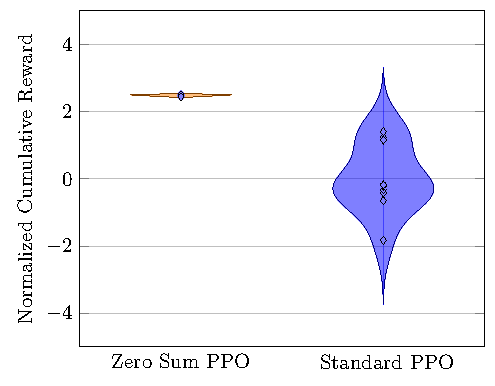
\includegraphics[width=.33\textwidth]{plots/ppo/violin_plot/initial_condition_shift.pdf}}%
	\subfloat[اغتشاش در عملگرها]{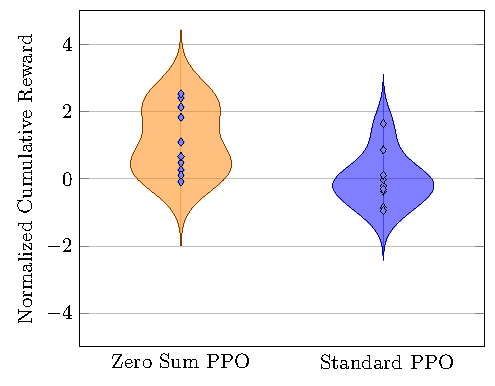
\includegraphics[width=.33\textwidth]{plots/ppo/violin_plot/actuator_disturbance.pdf}}%
	\subfloat[عدم تطابق مدل]{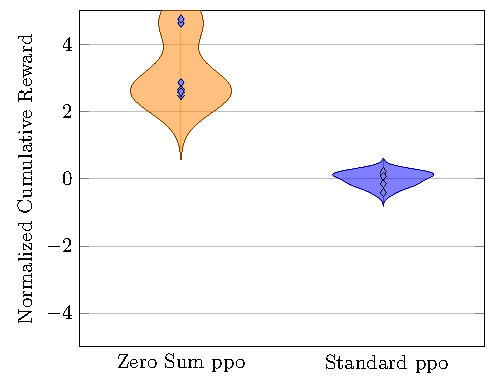
\includegraphics[width=.33\textwidth]{plots/ppo/violin_plot/model_mismatch.pdf}}\\[1ex]
	
	% سطر دوم
	\subfloat[مشاهده ناقص]{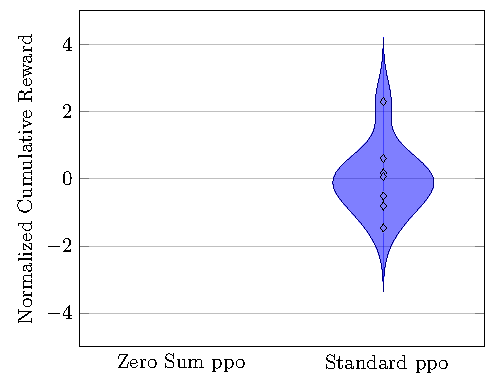
\includegraphics[width=.33\textwidth]{plots/ppo/violin_plot/partial_observation.pdf}}%
	\subfloat[نویز حسگر]{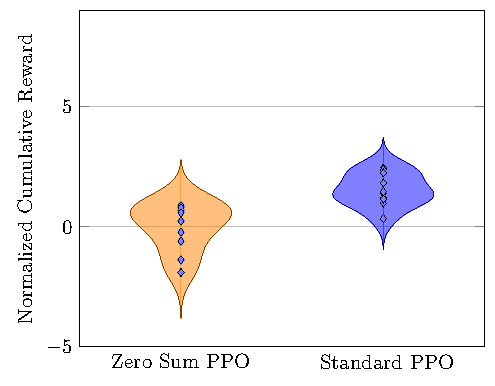
\includegraphics[width=.33\textwidth]{plots/ppo/violin_plot/sensor_noise.pdf}}%
	\subfloat[تأخیر زمانی]{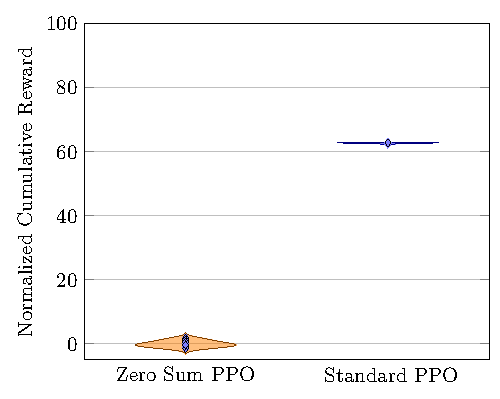
\includegraphics[width=.33\textwidth]{plots/ppo/violin_plot/time_delay.pdf}}
	
	\caption{مقایسه مجموع پاداش دو الگوریتم تک‌عاملی و چندعاملی \lr{PPO} در سناریوهای مختلف. 
%		نسخه بازی مجموع‌صفر در سناریوهای تأخیر زمانی و نویز حسگر برتری قابل توجهی نشان می‌دهد.
		}
	\label{fig:ppo_robustness_violin}
\end{figure}

الگوریتم \lr{PPO} در حالت بازی مجموع‌صفر در اکثر سناریوها عملکرد بهتری نشان می‌دهد، به خصوص در شرایط تأخیر زمانی و نویز حسگر. این می‌تواند نشان‌دهنده توانایی روش چندعاملی در مدیریت بهتر شرایط دارای عدم قطعیت در ورودی‌ها باشد. با این حال، تفاوت در برخی از سناریوها کمتر از \lr{DDPG} است.




\begin{table}
	\centering
	\setlength{\tabcolsep}{2pt}
	\small
	\begin{tabular}{@{} R{3.2cm} *{8}{C{1.05cm}} @{}}
		\toprule
		\multirow{2}{*}{\makecell[r]{سناریو}}
		& \multicolumn{2}{c}{پاداش تجمعی} & \multicolumn{2}{c}{مجموع خطای مسیر}
		& \multicolumn{2}{c}{مجموع تلاش کنترلی} & \multicolumn{2}{c}{احتمال شکست} \\
		\cmidrule(lr){2-3}\cmidrule(lr){4-5}\cmidrule(lr){6-7}\cmidrule(lr){8-9}
		& {\rotatebox[origin=c]{90}{\lr{PPO}}} & {\rotatebox[origin=c]{90}{\lr{MA-PPO}}}
		& {\rotatebox[origin=c]{90}{\lr{PPO}}} & {\rotatebox[origin=c]{90}{\lr{MA-PPO}}}
		& {\rotatebox[origin=c]{90}{\lr{PPO}}} & {\rotatebox[origin=c]{90}{\lr{MA-PPO}}}
		& {\rotatebox[origin=c]{90}{\lr{PPO}}} & {\rotatebox[origin=c]{90}{\lr{MA-PPO}}} \\
		\midrule
		شرایط اولیه تصادفی
		&
		$-1.85$ & $0.46$ & $0.22$ & $0.14$ & $1.98$ & $1.98$ & $0.70$ & $0.00$ \\
		اغتشاش در عملگرها
		&
		$-1.97$ & $-1.91$ & $8.33$ & $7.50$ & $3.42$ & $3.42$ & $1.00$ & $1.00$ \\
		عدم تطابق مدل
		&
		$0.46$ & $0.30$ & $0.07$ & $0.08$ & $1.13$ & $1.13$ & $0.00$ & $0.00$ \\
		مشاهده ناقص
		&
		$-3.60$ & $-1.81$ & $2.34$ & $2.06$ & $2.15$ & $2.15$ & $1.00$ & $1.00$ \\
		نویز حسگر  
		&
		$0.52$ & $0.48$ & $0.13$ & $0.15$ & $2.08$ & $2.08$ & $0.00$ & $0.00$ \\
		تأخیر زمانی        
		&
		$0.58$ & $-2.44$ & $0.03$ & $2.49$ & $2.56$ & $2.56$ & $0.00$ & $1.00$ \\
		\bottomrule
	\end{tabular}
	\caption{جدول پارامترها و مقادیر پیش‌فرض الگوریتم \lr{PPO}}
\end{table}









\subsection{مقایسه الگوریتم‌های تک‌عاملی و چندعاملی \lr{SAC}}

\begin{figure}[H]
	\centering
	
	% سطر اول
	\subfloat[شرایط اولیه تصادفی]{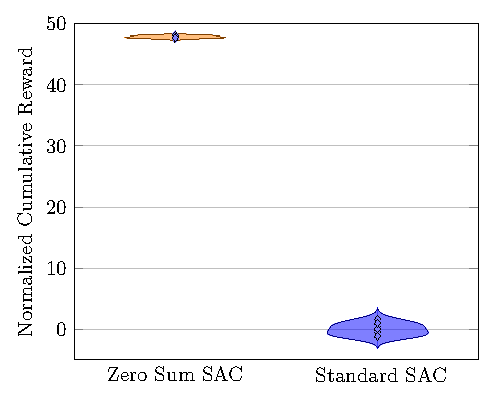
\includegraphics[width=.33\textwidth]{plots/sac/violin_plot/initial_condition_shift.pdf}}%
	\subfloat[اغتشاش در عملگرها]{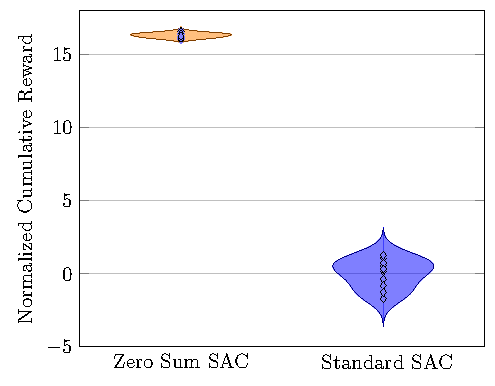
\includegraphics[width=.33\textwidth]{plots/sac/violin_plot/actuator_disturbance.pdf}}%
	\subfloat[عدم تطابق مدل]{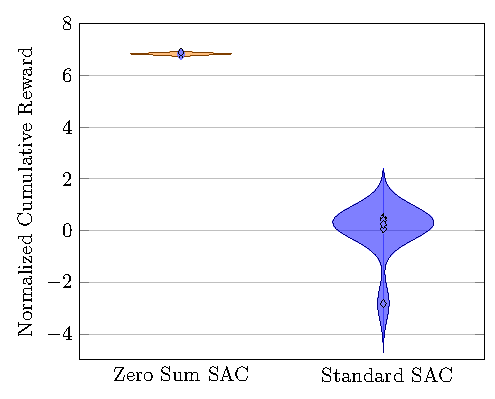
\includegraphics[width=.33\textwidth]{plots/sac/violin_plot/model_mismatch.pdf}}\\[1ex]
	
	% سطر دوم
	\subfloat[مشاهده ناقص]{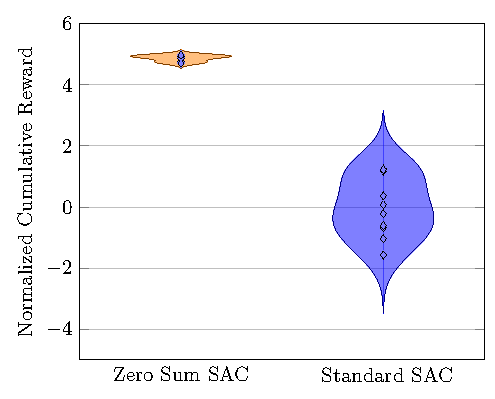
\includegraphics[width=.33\textwidth]{plots/sac/violin_plot/partial_observation.pdf}}%
	\subfloat[نویز حسگر]{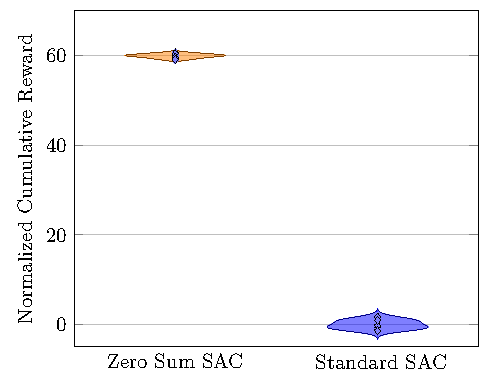
\includegraphics[width=.33\textwidth]{plots/sac/violin_plot/sensor_noise.pdf}}%
	\subfloat[تأخیر زمانی]{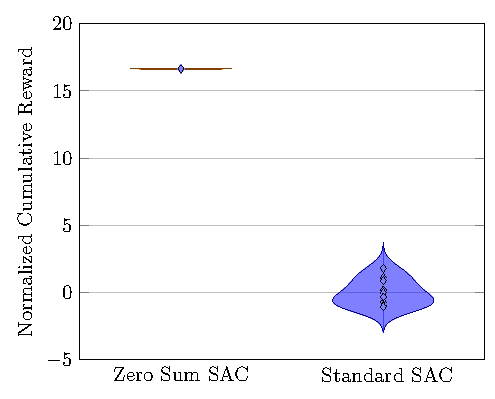
\includegraphics[width=.33\textwidth]{plots/sac/violin_plot/time_delay.pdf}}
	
	\caption{مقایسه مجموع پاداش دو الگوریتم تک‌عاملی و چندعاملی \lr{SAC} در سناریوهای مختلف. 
%		هر دو نسخه عملکرد نسبتاً خوبی دارند، اما نسخه بازی مجموع‌صفر در شرایط عدم تطابق مدل و مشاهده ناقص برتری بیشتری نشان می‌دهد.
}
	\label{fig:sac_robustness_violin}
\end{figure}

الگوریتم \lr{SAC} در هر دو حالت عملکرد نسبتاً خوبی در سناریوهای مختلف نشان می‌دهد. این می‌تواند به دلیل استفاده از مکانیزم آنتروپی باشد که به صورت ذاتی اکتشاف بیشتری را تشویق می‌کند. با این حال، نسخه بازی مجموع‌صفر در تمامی سناریوها  برتری معناداری دارد که نشان‌دهنده مقاومت بیشتر آن در شرایط با اطلاعات محدود است.







\begin{table}
	\centering
	\setlength{\tabcolsep}{2pt}
	\small
	\begin{tabular}{@{} R{3.2cm} *{8}{C{1.05cm}} @{}}
		\toprule
		\multirow{2}{*}{\makecell[r]{سناریو}}
		& \multicolumn{2}{c}{پاداش تجمعی} & \multicolumn{2}{c}{مجموع خطای مسیر}
		& \multicolumn{2}{c}{مجموع تلاش کنترلی} & \multicolumn{2}{c}{احتمال شکست} \\
		\cmidrule(lr){2-3}\cmidrule(lr){4-5}\cmidrule(lr){6-7}\cmidrule(lr){8-9}
		& {\rotatebox[origin=c]{90}{\lr{SAC}}} & {\rotatebox[origin=c]{90}{\lr{MA-SAC}}}
		& {\rotatebox[origin=c]{90}{\lr{SAC}}} & {\rotatebox[origin=c]{90}{\lr{MA-SAC}}}
		& {\rotatebox[origin=c]{90}{\lr{SAC}}} & {\rotatebox[origin=c]{90}{\lr{MA-SAC}}}
		& {\rotatebox[origin=c]{90}{\lr{SAC}}} & {\rotatebox[origin=c]{90}{\lr{MA-SAC}}} \\
		\midrule
		شرایط اولیه تصادفی
		&
		&&&&&&& \\
		اغتشاش در عملگرها
		&
		&&&&&&& \\
		عدم تطابق مدل
		&
		&&&&&&& \\
		مشاهده ناقص
		&
		&&&&&&& \\
		نویز حسگر  
		&
		&&&&&&& \\
		تأخیر زمانی        
		&
		&&&&&&& \\
		\bottomrule
	\end{tabular}
	\caption{جدول پارامترها و مقادیر پیش‌فرض الگوریتم \lr{SAC}}
\end{table}














\subsection{مقایسه الگوریتم‌های تک‌عاملی و چندعاملی \lr{TD3}}

\begin{figure}[H]
	\centering
	
	% سطر اول
	\subfloat[شرایط اولیه تصادفی]{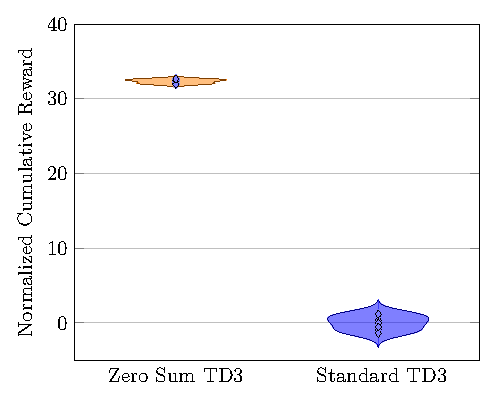
\includegraphics[width=.33\textwidth]{plots/td3/violin_plot/initial_condition_shift.pdf}}%
	\subfloat[اغتشاش در عملگرها]{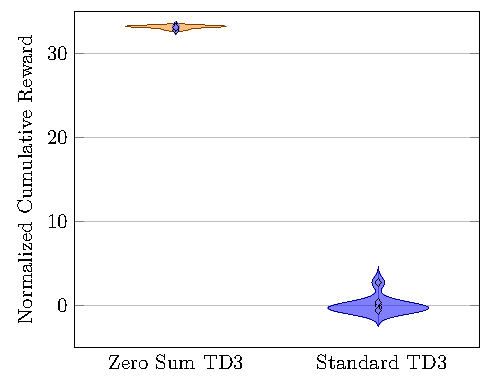
\includegraphics[width=.33\textwidth]{plots/td3/violin_plot/actuator_disturbance.pdf}}%
	\subfloat[عدم تطابق مدل]{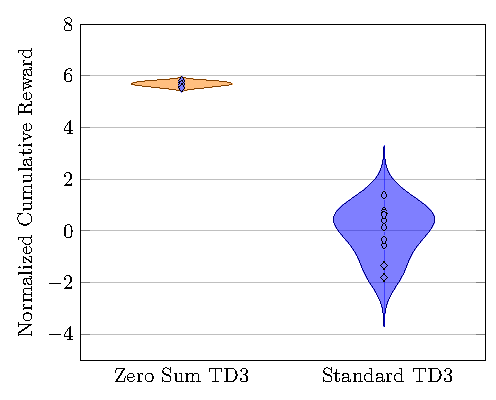
\includegraphics[width=.33\textwidth]{plots/td3/violin_plot/model_mismatch.pdf}}\\[1ex]
	
	% سطر دوم
	\subfloat[مشاهده ناقص]{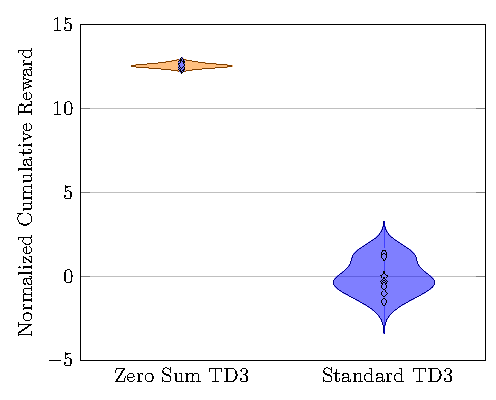
\includegraphics[width=.33\textwidth]{plots/td3/violin_plot/partial_observation.pdf}}%
	\subfloat[نویز حسگر]{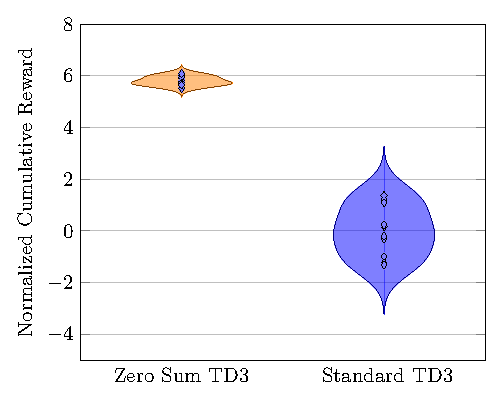
\includegraphics[width=.33\textwidth]{plots/td3/violin_plot/sensor_noise.pdf}}%
	\subfloat[تأخیر زمانی]{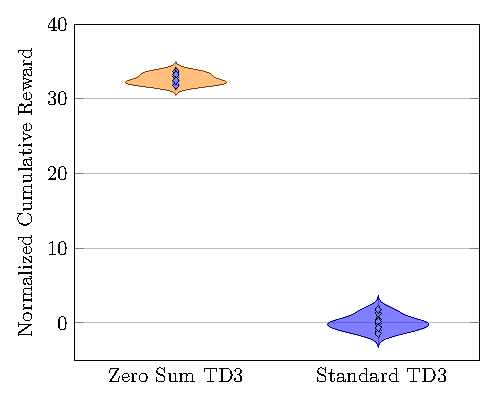
\includegraphics[width=.33\textwidth]{plots/td3/violin_plot/time_delay.pdf}}
	
	\caption{مقایسه مجموع پاداش دو الگوریتم تک‌عاملی و چندعاملی \lr{TD3} در سناریوهای مختلف. 
%		نسخه بازی مجموع‌صفر در تمام سناریوها عملکرد بهتری را نشان می‌دهد، با برتری قابل توجه در سناریوهای اغتشاش در عملگرها و نویز حسگر.
		}
	\label{fig:td3_robustness_violin}
\end{figure}

الگوریتم \lr{TD3} مبتنی بر بازی مجموع‌صفر در تمامی سناریوها نشان می‌دهد. 
%این برتری در سناریوهای اغتشاش در عملگرها و نویز حسگر بسیار قابل توجه است. 
این نتایج نشان می‌دهد که ترکیب مکانیزم‌های پایدارسازی \lr{TD3} با رویکرد بازی مجموع‌صفر می‌تواند منجر به مقاومت قابل توجهی در برابر شرایط نامطلوب شود.

\section{مقایسه جامع الگوریتم‌ها}
\label{sec:comprehensive_comparison}

در این بخش، مقایسه جامعی بین تمام الگوریتم‌ها در دو حالت تک‌عاملی و چندعاملی ارائه شده است. هدف، تعیین بهترین الگوریتم برای هر سناریوی خاص و درک بهتر نقاط قوت و ضعف هر روش است.

\subsection{مقایسه الگوریتم‌های تک‌عاملی}

\begin{figure}[H]
	\centering

	% سطر اول
	\subfloat[شرایط اولیه تصادفی]{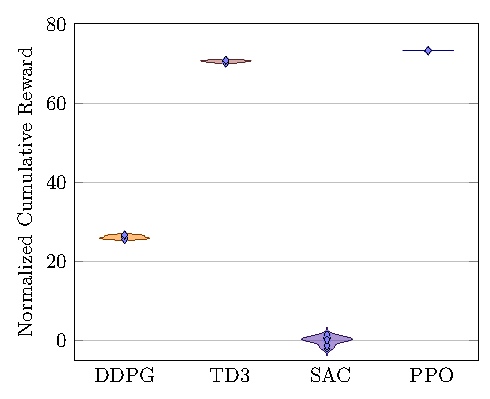
\includegraphics[width=.33\textwidth]{plots/standard/violin_plot/initial_condition_shift.pdf}}%
	\subfloat[اغتشاش در عملگرها]{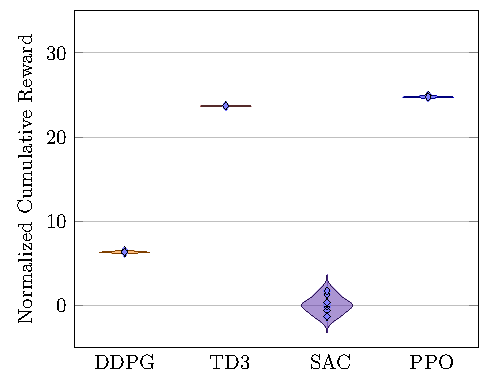
\includegraphics[width=.33\textwidth]{plots/standard/violin_plot/actuator_disturbance.pdf}}%
	\subfloat[عدم تطابق مدل]{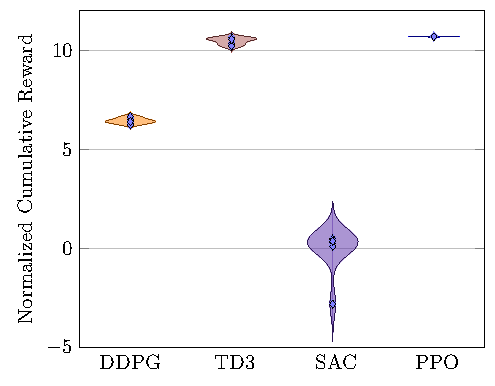
\includegraphics[width=.33\textwidth]{plots/standard/violin_plot/model_mismatch.pdf}}\\[1ex]

	% سطر دوم
	\subfloat[مشاهده ناقص]{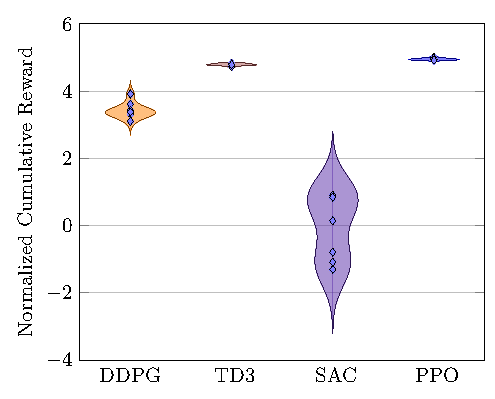
\includegraphics[width=.33\textwidth]{plots/standard/violin_plot/partial_observation.pdf}}%
	\subfloat[نویز حسگر]{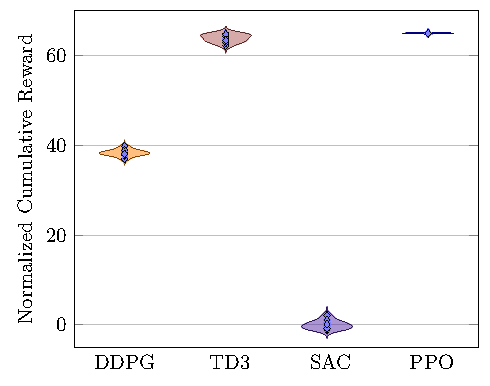
\includegraphics[width=.33\textwidth]{plots/standard/violin_plot/sensor_noise.pdf}}%
	\subfloat[تأخیر زمانی]{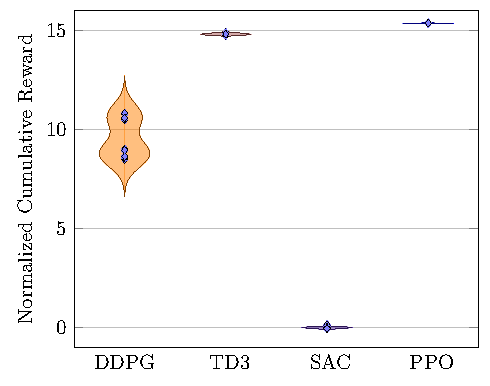
\includegraphics[width=.33\textwidth]{plots/standard/violin_plot/time_delay.pdf}}

	\caption{مقایسه مجموع پاداش الگوریتم‌های تک‌عاملی در سناریوهای مختلف.}
	\label{fig:all_solo_robustness_violin}
\end{figure}

در میان الگوریتم‌های تک‌عاملی، \lr{PPO} و \lr{TD3} در اکثر سناریوها عملکرد بهتری نسبت به \lr{DDPG} و \lr{SAC} نشان می‌دهند.
% \lr{PPO} به طور خاص در سناریوهای نویز حسگر و تأخیر زمانی برتری قابل توجهی دارد که می‌تواند به دلیل استفاده از مکانیزم آنتروپی و توانایی آن در حفظ تعادل بین اکتشاف و بهره‌برداری باشد. \lr{TD3} نیز در شرایط عدم تطابق مدل و اغتشاش در عملگرها عملکرد قابل توجهی ارائه می‌دهد.

\subsection{مقایسه الگوریتم‌های چندعاملی}

\begin{figure}[H]
	\centering

	% سطر اول
	\subfloat[شرایط اولیه تصادفی]{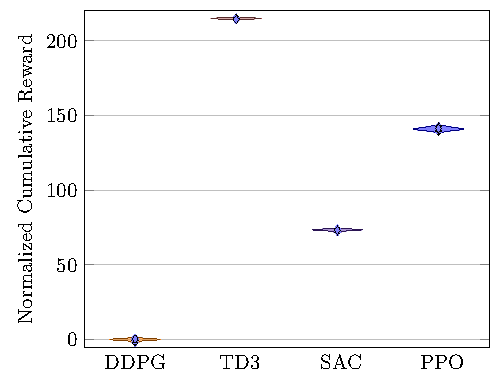
\includegraphics[width=.33\textwidth]{plots/ZeroSum/violin_plot/initial_condition_shift.pdf}}%
	\subfloat[اغتشاش در عملگرها]{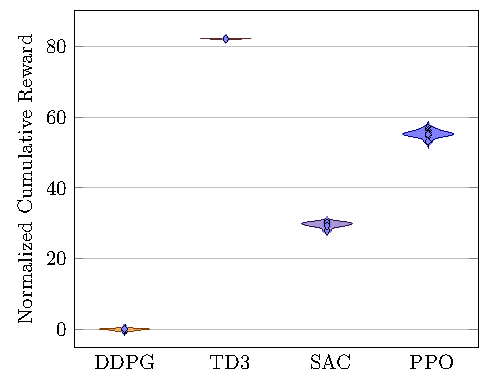
\includegraphics[width=.33\textwidth]{plots/ZeroSum/violin_plot/actuator_disturbance.pdf}}%
	\subfloat[عدم تطابق مدل]{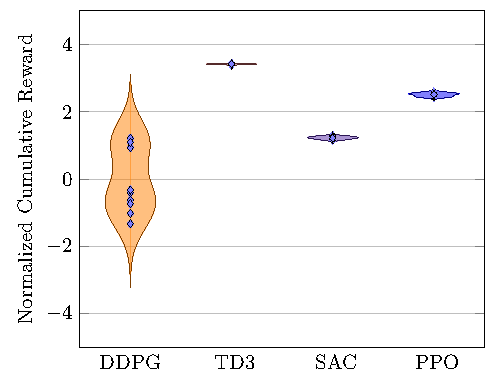
\includegraphics[width=.33\textwidth]{plots/ZeroSum/violin_plot/model_mismatch.pdf}}\\[1ex]

	% سطر دوم
	\subfloat[مشاهده ناقص]{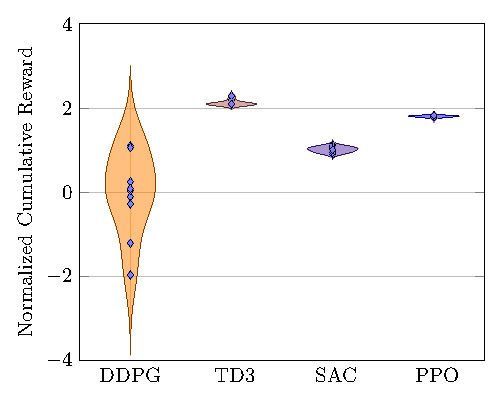
\includegraphics[width=.33\textwidth]{plots/ZeroSum/violin_plot/partial_observation.pdf}}%
	\subfloat[نویز حسگر]{\includegraphics[width=.33\textwidth]{plots/ZeroSum/violin_plot/sensor_noise.pdf}}%
	\subfloat[تأخیر زمانی]{\includegraphics[width=.33\textwidth]{plots/ZeroSum/violin_plot/time_delay.pdf}}

	\caption{مقایسه مجموع پاداش الگوریتم‌های چندعاملی در سناریوهای مختلف.}
	\label{fig:all_multi_robustness_violin}
\end{figure}

در میان الگوریتم‌های تک‌عاملی، \lr{PPO} و \lr{TD3} در اکثر سناریوها عملکرد بهتری نسبت به \lr{DDPG} و \lr{SAC} نشان می‌دهند.

\section{تحلیل پایداری و همگرایی}
\label{sec:stability_analysis}

پایداری و سرعت همگرایی فرآیند یادگیری با استفاده از نمودارهای پاداش و معیارهای عددی مورد بررسی قرار گرفته است. نتایج نشان می‌دهد که الگوریتم‌های مبتنی بر بازی مجموع‌صفر در اکثر موارد همگرایی پایدارتری را نسبت به نسخه‌های استاندارد نشان می‌دهند. این پایداری به خصوص در \lr{TD3} و \lr{PPO} قابل توجه است.

تحلیل نرخ همگرایی نشان می‌دهد که \lr{PPO} در هر دو نسخه استاندارد و بازی مجموع‌صفر، سریع‌ترین همگرایی را دارد، در حالی که \lr{DDPG} کندترین نرخ را نشان می‌دهد. با این حال، کیفیت نهایی سیاست آموخته‌شده در \lr{TD3} مبتنی بر بازی مجموع‌صفر بالاترین است.

\section{مقایسه با معیارهای مرجع}
\label{sec:benchmark_comparison}

عملکرد الگوریتم‌ها با روش‌های مرجع مانند کنترل بهینه کلاسیک و کنترل پیش‌بین مدل مقایسه شده تا برتری‌ها و محدودیت‌های آن‌ها مشخص گردد. نتایج نشان می‌دهد که در شرایط ایده‌آل، روش‌های کنترل بهینه کلاسیک دقت بالاتری دارند، اما در حضور عدم قطعیت‌ها و اختلالات، الگوریتم‌های یادگیری تقویتی به خصوص نسخه‌های مبتنی بر بازی مجموع‌صفر، مقاومت و انعطاف‌پذیری بیشتری نشان می‌دهند.

در مجموع، الگوریتم \lr{TD3} مبتنی بر بازی مجموع‌صفر بهترین تعادل بین دقت، کارایی و مقاومت را در مقایسه با سایر روش‌ها و معیارهای مرجع ارائه می‌دهد.










%
%
%
%\begin{table}
%	\centering
%	\begin{tabular}{c|c|c|c|c|c|c|c|c|}
%		\cline{2-9}
%		& \multicolumn{4}{c|}{یادگیری تقویتی چندعاملی} & \multicolumn{4}{c|}{یادگیری تقویتی تک‌عاملی}
%		
%		\\
%		\hline
%		\multicolumn{1}{|c|}{معیار عملکرد} 
%		&
%		\lr{MA-DDPG} 
%		&
%		\lr{MA-TD3} 
%		&
%	\lr{MA-PPO} 
%		&
%	\lr{MA-SAC} 
%		&
%		\lr{DDPG} 
%		&
%		\lr{TD3} 
%		&
%		\lr{PPO} 
%		&
%		\lr{SAC} 
%		\\
%		\hline
%		\multicolumn{1}{|c|}{
%			پاداش تجمی
%		}
%		&&&&&&&&
%	\end{tabular}
%\end{table}
%
%
%
%
%
%
%
%\begin{table}
%	\centering
%	\setlength{\tabcolsep}{2.5pt} % default is ~6pt; smaller = tighter columns
%	\begin{tabular}{c|c|c|c|c|c|c|c|c|}
%		\cline{2-9}
%		& \multicolumn{2}{c|}{پاداش} & \multicolumn{2}{c|}{پاداش} & \multicolumn{2}{c|}{پاداش} & \multicolumn{2}{c|}{پاداش}
%		
%		\\
%		\hline
%		%		1 & 2 & 3&4&5&6&7&8&9\\
%		\multicolumn{1}{|c|}{سناریو} 
%		&
%		\lr{DDPG} 
%		&
%		\lr{MA-DDPG} 
%		&
%	\lr{DDPG} 
%		&
%		\lr{MA-DDPG} 
%		&
%		\lr{DDPG}  
%		&
%		\lr{MA-DDPG} 
%		&
%	\lr{DDPG} 
%		&
%		\lr{MA-DDPG} 
%		\\
%		\hline
%	\end{tabular}
%\end{table}
%
%
%
%
%
%
%% Preamble (once)
%
%
%% Table
%\begin{table}
%	\centering
%	\setlength{\tabcolsep}{2pt} % tighter inner padding
%	\small                      % slightly smaller font (nice width win)
%	
%	\begin{tabular}{@{} R{2.2cm} *{8}{C{1.05cm}} @{}}
%		\toprule
%		& \multicolumn{2}{c}{پاداش ۱} & \multicolumn{2}{c}{پاداش ۲}
%		& \multicolumn{2}{c}{پاداش ۳} & \multicolumn{2}{c}{پاداش ۴} \\
%		\cmidrule(lr){2-3}\cmidrule(lr){4-5}\cmidrule(lr){6-7}\cmidrule(lr){8-9}
%		\makecell[r]{سناریو}
%		& {\rotatebox[origin=c]{90}{\lr{DDPG}}}    & {\rotatebox[origin=c]{90}{\lr{MA-DDPG}}}
%		& {\rotatebox[origin=c]{90}{\lr{DDPG}}}    & {\rotatebox[origin=c]{90}{\lr{MA-DDPG}}}
%		& {\rotatebox[origin=c]{90}{\lr{DDPG}}}    & {\rotatebox[origin=c]{90}{\lr{MA-DDPG}}}
%		& {\rotatebox[origin=c]{90}{\lr{DDPG}}}    & {\rotatebox[origin=c]{90}{\lr{MA-DDPG}}} \\
%		\midrule
%		% ... rows ...
%		\bottomrule
%	\end{tabular}
%\end{table}
%
%
%
%\begin{table}
%	\centering
%%	\setlength{\tabcolsep}{2.5pt}
%%	\renewcommand{\arraystretch}{0.95}
%	
%	\begin{tabular}{@{} R{2.2cm} *{8}{C{1.05cm}} @{}}
%	\toprule
%	& \multicolumn{2}{c}{پاداش ۱} & \multicolumn{2}{c}{پاداش ۲}
%	& \multicolumn{2}{c}{پاداش ۳} & \multicolumn{2}{c}{پاداش ۴} \\
%	\cmidrule(lr){2-3}\cmidrule(lr){4-5}\cmidrule(lr){6-7}\cmidrule(lr){8-9}
%	\makecell[r]{سناریو}
%	& {\rotatebox[origin=c]{90}{\lr{DDPG}}}    & {\rotatebox[origin=c]{90}{\lr{MA-DDPG}}}
%	& {\rotatebox[origin=c]{90}{\lr{DDPG}}}    & {\rotatebox[origin=c]{90}{\lr{MA-DDPG}}}
%	& {\rotatebox[origin=c]{90}{\lr{DDPG}}}    & {\rotatebox[origin=c]{90}{\lr{MA-DDPG}}}
%	& {\rotatebox[origin=c]{90}{\lr{DDPG}}}    & {\rotatebox[origin=c]{90}{\lr{MA-DDPG}}} \\
%		\hline
%		\multicolumn{1}{|c|}{شرایط اولیه تصادفی} & & & & & & & & \\ \hline
%		\multicolumn{1}{|c|}{اغتشاش در عملگرها}   & & & & & & & & \\ \hline
%		\multicolumn{1}{|c|}{عدم تطابق مدل}       & & & & & & & & \\ \hline
%		\multicolumn{1}{|c|}{مشاهده ناقص}         & & & & & & & & \\ \hline
%		\multicolumn{1}{|c|}{نویز حسگر}            & & & & & & & & \\ \hline
%		\multicolumn{1}{|c|}{تأخیر زمانی}          & & & & & & & & \\ \hline
%	\end{tabular}
%\end{table}
%
%
%
%
%\begin{table}
%	\centering
%	\setlength{\tabcolsep}{2pt}
%	\small
%	\begin{tabular}{@{} R{2.2cm} *{8}{C{1.05cm}} @{}}
%		\toprule
%		& \multicolumn{2}{c}{پاداش ۱} & \multicolumn{2}{c}{پاداش ۲}
%		& \multicolumn{2}{c}{پاداش ۳} & \multicolumn{2}{c}{پاداش ۴} \\
%		\cmidrule(lr){2-3}\cmidrule(lr){4-5}\cmidrule(lr){6-7}\cmidrule(lr){8-9}
%		\makecell[r]{سناریو}
%		& {\rotatebox[origin=c]{90}{\lr{DDPG}}}    & {\rotatebox[origin=c]{90}{\lr{MA-DDPG}}}
%		& {\rotatebox[origin=c]{90}{\lr{DDPG}}}    & {\rotatebox[origin=c]{90}{\lr{MA-DDPG}}}
%		& {\rotatebox[origin=c]{90}{\lr{DDPG}}}    & {\rotatebox[origin=c]{90}{\lr{MA-DDPG}}}
%		& {\rotatebox[origin=c]{90}{\lr{DDPG}}}    & {\rotatebox[origin=c]{90}{\lr{MA-DDPG}}} \\
%		\midrule
%		شرایط اولیه تصادفی & & & & & & & & \\
%		اغتشاش در عملگرها & & & & & & & & \\
%		عدم تطابق مدل     & & & & & & & & \\
%		مشاهده ناقص       & & & & & & & & \\
%		نویز حسگر          & & & & & & & & \\
%		تأخیر زمانی        & & & & & & & & \\
%		\bottomrule
%	\end{tabular}
%\end{table}



% Preamble (once)
% \usepackage{array,booktabs,makecell,multirow,graphicx}
% \newcolumntype{R}[1]{>{\raggedleft\arraybackslash}p{#1}}
% \newcolumntype{C}[1]{>{\centering\arraybackslash}p{#1}}


\begin{table}
	\centering
	\setlength{\tabcolsep}{2pt}
	\small
	\begin{tabular}{@{} R{3.2cm} *{8}{C{1.05cm}} @{}}
		\toprule
		\multirow{2}{*}{\makecell[r]{سناریو}}
		& \multicolumn{2}{c}{پاداش تجمعی} & \multicolumn{2}{c}{مجموع خطای مسیر}
		& \multicolumn{2}{c}{مجموع تلاش کنترلی} & \multicolumn{2}{c}{احتمال شکست} \\
		\cmidrule(lr){2-3}\cmidrule(lr){4-5}\cmidrule(lr){6-7}\cmidrule(lr){8-9}
		& {\rotatebox[origin=c]{90}{\lr{DDPG}}} & {\rotatebox[origin=c]{90}{\lr{MA-DDPG}}}
		& {\rotatebox[origin=c]{90}{\lr{DDPG}}} & {\rotatebox[origin=c]{90}{\lr{MA-DDPG}}}
		& {\rotatebox[origin=c]{90}{\lr{DDPG}}} & {\rotatebox[origin=c]{90}{\lr{MA-DDPG}}}
		& {\rotatebox[origin=c]{90}{\lr{DDPG}}} & {\rotatebox[origin=c]{90}{\lr{MA-DDPG}}} \\
		\midrule
		شرایط اولیه تصادفی
		&
		&&&&&&& \\
		اغتشاش در عملگرها
		&
		&&&&&&& \\
		عدم تطابق مدل
		&
		&&&&&&& \\
		مشاهده ناقص
		&
		&&&&&&& \\
		نویز حسگر  
		&
		&&&&&&& \\
		تأخیر زمانی        
		&
		&&&&&&& \\
		\bottomrule
	\end{tabular}
	\caption{جدول پارامترها و مقادیر پیش‌فرض الگوریتم \lr{PPO}}
\end{table}

